\makeatletter
\def\input@path{{../styles/}{../../styles/}{../../../styles/}{../}{../../}{../../../}}
\makeatother


\documentclass{ee102_pset}
\input{macros.tex}
\input{preamble.tex}

% Assignment info
\author{\rule{3cm}{0.4pt}} % Name placeholder
\submitdate{\rule{3cm}{0.4pt}} % Submission date placeholder
\problemset{Problem Set \#6: Fourier Series}
\renewcommand{\psetnum}{6}
\renewcommand{\releasedate}{October 5, 2026}
\renewcommand{\duedate}{October 14, 2026}
\shorttitle{Problem Set \#6}
\hypersetup{pdftitle={EE 102 Problem Set 6: Fourier Series}}

\begin{document}
\problem{1}
Consider the RC circuit from Pre-requisite \#3, with input voltage
$x(t)$ and output voltage $y(t)$ measured across the capacitor. Use
$R=330\,\Omega$ and $C=1000\,\mu\mathrm{F}$, so $RC=0.33\,\mathrm{s}$.
Its impulse response is
\[
h(t)=\frac{1}{RC}e^{-t/(RC)}u(t).
\]
For each of the input signals below, find the Fourier series representation
of the \textbf{periodic steady-state output} $y(t)$.

\problempart[20 points] A train of impulses:
\[
x(t) = \sum_{n=-\infty}^{\infty} \delta(t - n)
\]


\textbf{Hint:} Start by finding the Fourier series representation of the input signal, $x(t)$. So, write
\[ x(t) = \sum_{k=-\infty}^{\infty} a_k e^{jk\omega_0 t}, \]
where $\omega_0 = 2\pi/T$ is the fundamental frequency and $T$ is the period of the input signal. Find $a_k$ using the Fourier series analysis equation. Then, use the property of LTI systems to find the output coefficients $b_k$ (that is, the Fourier Series coefficients of the output signal) in terms of the input coefficients $a_k$.
\[
b_k = a_k H(jk\omega_0),
\]
where $H(j\omega)$ is the frequency response of the system. Refer to the lecture notes to find out the frequency response formula!

\problempart[30 points] A square wave of amplitude 1 sketched below in Figure~\ref{fig:square_wave}.
\begin{figure}[h]
  \centering
  \begin{tikzpicture}[x=1.2cm,y=1.2cm,line cap=round]
  \pgfmathsetmacro{\H}{1}      % unit pulse height
  \pgfmathsetmacro{\W}{0.5}    % pulse width
  \pgfmathsetmacro{\hh}{0.5*\W}

  % axis
  \draw[->] (-3.6,0)--(4.6,0) node[below] {$t$};

  % pulses centered at integers
  \foreach \n in {-3,-2,-1,0,1,2,3,4}{
    \draw (\n-\hh,0) -- (\n-\hh,\H) -- (\n+\hh,\H) -- (\n+\hh,0);
  }

  % integer ticks and labels
  \foreach \n in {-3,-2,-1,0,1,2,3,4}{
    \draw (\n,0) -- ++(0,-0.06) node[below=2pt] {\small \n};
  }

  % ellipses at ends
  \node at (-3.9,0.58) {$\cdots$};
  \node at ( 4.8,0.58) {$\cdots$};

  % label x(t) over the n=0 pulse
  \draw[->] (0,-0.05) -- (0,\H+0.45);
  \node[left] at (0,\H) {$1$};
  \node at (0,\H+0.75) {$x(t)$};

  % show width = 1/2 above the pulse at t=1
  \draw[<->] (1-\hh,\H+0.25) -- (1+\hh,\H+0.25)
    node[midway,fill=white,inner sep=1pt] {$\tfrac{1}{2}$};
\end{tikzpicture}
\caption{A square wave of amplitude $1$, period $T=1$, and duty cycle $50\%$.}
\label{fig:square_wave}


\end{figure}

Hint: Over one period, $-\tfrac12\le t<\tfrac12$, the signal is
\[
x(t)=
\begin{cases}
1, & -\tfrac14\le t\le\tfrac14,\\
0, & \text{otherwise within this period.}
\end{cases}
\]

% \problempart[20 points] The input $x(t)$ in part (b) models a PWM signal
% with a fixed duty cycle. Double its switching frequency while keeping
% the amplitude and duty cycle unchanged:
% \[
% x_{\mathrm{new}}(t)=x(2t).
% \]
% Sketch this new input and state its fundamental period. Use the Fourier
% series coefficients from part (b), the time-scaling property, and the LTI
% system's response at the new harmonic frequencies to find the Fourier
% series representation of the new output.

% Hint: Time scaling changes the harmonic frequencies while retaining the
% input coefficient sequence.You do not need to recompute the input coefficients
% from scratch. Instead, start by writing:


\problempart[20 points] Write Python/MATLAB code to implement the input
signals above. Compute the outputs and their Fourier series representations,
and plot the magnitude of the outputs, $|y(t)|$, on a graph.

Note that you will need to choose a finite number of harmonics to include in the Fourier series representation (computers cannot handle infinite sums!). Additionally, you will need to choose a sampling interval for your simulation.

You may use AI tools to get help with the syntax and to get a set up going -- you must write your own Fourier series computation code though.


% Validate your analytical
% results against simulations in periodic steady state, after startup
% transients have decayed. State your sampling interval and the number of
% harmonics used.

\problem{2}
Compute the complex Fourier series representation of each signal below.
For each signal $f(t)$, let $c_k$ be its Fourier series coefficients and
$\omega_0=2\pi/T_0$. Define the truncated representation by
\[
f_N(t)=\sum_{k=-N}^{N}c_k e^{jk\omega_0t}.
\]
Thus, retain the DC term and the first $N$ positive and negative harmonics.
For $N=1,2,3,4$, compute the error energy \textbf{over one period}:
\[
E_N=\int_0^{T_0}\left|f(t)-f_N(t)\right|^2\,dt.
\]
You may use computer programs for computations. Show how you obtain the
coefficients and the error energy.

\problempart[15 points] A sawtooth signal with fundamental period $T_0=1$.
Figure~\ref{fig:problem2}(a) shows one period:
\[
x(t)=t,\qquad 0\le t<1,\qquad x(t+1)=x(t).
\]
Extend this definition periodically to all positive and negative time.

Hint: Evaluate the coefficient integral over $0\le t<1$. Integration by parts can be useful for the nonzero harmonics.
\problempart[15 points]
A rectangular signal with fundamental period $T_0=2$, shown in
Figure~\ref{fig:problem2}(b). Over one period,
\[
y(t)=
\begin{cases}
1, & 0\le t<1,\\
0, & 1\le t<2,
\end{cases}
\qquad y(t+2)=y(t).
\]
The signal repeats periodically for all positive and negative time.

\begin{figure}[h]
\centering
  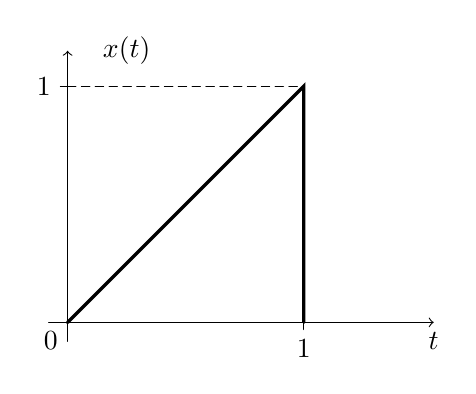
\begin{tikzpicture}[x=3.0cm,y=3.0cm,line cap=round]
\def\R{1.55}  % right extent
% axes
\draw[->] (-0.08,0)--(\R,0) node[below] {$t$};
\draw[->] (0,-0.08)--(0,1.15);
% ticks
\draw (0,1) -- ++(-0.03,0) node[left] {1};
\draw (1,0) -- ++(0,-0.03) node[below] {1};
\node[below left] at (0,0) {0};
% signal x(t): ramp on [0,1], drop, then 0
\draw[very thick] (0,0) -- (1,1) -- (1,0);
% guide at y=1
\draw[densely dashed] (0,1) -- (1,1);
% label
\node[above] at (0.25,1.05) {$x(t)$};
\end{tikzpicture}
\hspace{1.2cm}
% Figure (b): y(t)
\begin{tikzpicture}[x=3.0cm,y=3.0cm,line cap=round]
\def\R{2.5}
% axes
\draw[->] (-0.08,0)--(\R,0) node[below] {$t$};
\draw[->] (0,-0.08)--(0,1.15);
% ticks
\draw (0,1) -- ++(-0.03,0) node[left] {1};
\draw (1,0) -- ++(0,-0.03) node[below] {1};
\draw (2,0) -- ++(0,-0.03) node[below] {2};
\node[below left] at (0,0) {0};
% signal y(t): unit rectangle on [0,1]
\draw[very thick] (0,0) -- (0,1) -- (1,1) -- (1,0) -- (2,0);
% label
\node[above] at (0.18,1.05) {$y(t)$};
\end{tikzpicture}
\caption{One period of (a) the sawtooth signal $x(t)$ and (b) the rectangular signal $y(t)$.}
\label{fig:problem2}
\end{figure}

\end{document}
